\section{GP-MP Algorithm}
\label{sec:overall}

\subsection{Overall Algorithm}
\label{sec:schedule}

The proposed generative-prior message-passing receiver, denoted by GP-MP,
combines MFLE in Section~\ref{sec:linear-estimation} with GPJD.
The learned denoiser and activity classifier in
Section~\ref{sec:learning} implement the channel and activity updates
within GPJD, as illustrated in Fig.~\ref{fig:learned-receiver}.

\begin{figure*}[!t]
\centering
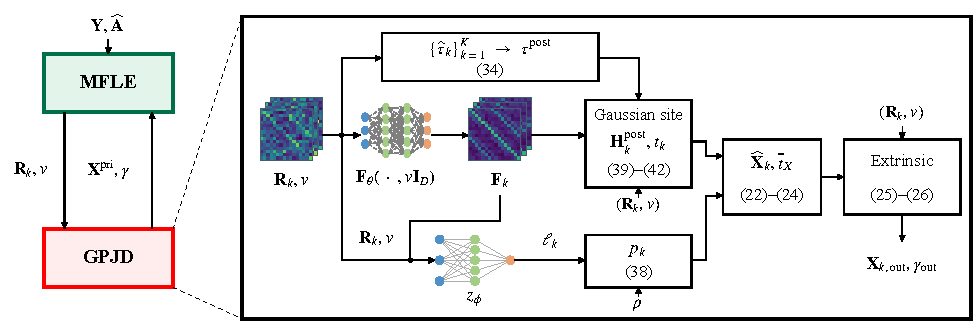
\includegraphics[width=0.92\textwidth]{learned_receiver.pdf}
\caption{Message exchange between MFLE and GPJD, with an expanded view of GPJD.
Following \cite[Fig.~3]{cai2026}, the denoising illustration uses an input--output
pair with a common magnitude scale.}
\label{fig:learned-receiver}
\end{figure*}

For an input Gaussian message with mean $\mathbf R_k$ and variance $v$,
the denoiser provides the channel mean
$\mathbf F_k=\mathbf F_\theta(\mathbf R_k,v)$ and the derivative-based
variance estimate $\widehat\tau_k=\widehat\tau_\theta(\mathbf R_k,v)$
in \eqref{eq:derivative-trace}.
The common variance $\tau^{\rm post}$ is the average of
$\widehat\tau_k$ over $k$, subject to the positive lower bound
$\tau_{\min}$. The classifier provides the corresponding activity
probability $p_k$ through \eqref{eq:activity-probability}.

Within GPJD, the channel prior is approximated by a Gaussian site
$\CN(\vect(\mathbf H_k);\vect(\mathbf E_k),\tau_k^{\rm ext}\I_D)$ \cite[Sec.~2.1]{vehtari2020}.
Its parameters follow from dividing the Gaussian posterior approximation,
with mean $\mathbf F_k$ and variance $\tau^{\rm post}$, by the input
likelihood:
\begin{align}
 \tau_k^{\rm ext}&=((\tau^{\rm post})^{-1}-v^{-1})^{-1},
 \label{eq:site-update}\\
 \mathbf E_k&=\tau_k^{\rm ext}\left(\frac{\mathbf F_k}{\tau^{\rm post}}-\frac{\mathbf R_k}{v}\right).
 \label{eq:site-mean}
\end{align}
The product of this site and the current Gaussian likelihood determines
the channel variance and mean under the active hypothesis:
\begin{align}
 t_k&=\frac{\tau_k^{\rm ext}v}{\tau_k^{\rm ext}+v},
 \label{eq:conditional-moments}\\
 \mathbf H_k^{\rm post}&=\frac{\tau_k^{\rm ext}\mathbf R_k+v\mathbf E_k}{\tau_k^{\rm ext}+v}.
 \label{eq:conditional-channel-mean}
\end{align}

Together with $p_k$, these moments determine the joint channel estimate
and the Gaussian extrinsic message returned to MFLE.
Algorithm~\ref{alg:gp-mp-ccd} summarizes the resulting iterations.
The receiver uses phases that are either available or estimated once
before MP by the method in Section~\ref{sec:phase-estimation}; they
remain fixed throughout the iterations.
Initialization uses the normalized training-channel power
$\widehat P_H$, defined as the average of $\norm{\mathbf H}_F^2/D$
over the training channels. Stopping checks and numerical settings
are given in Section~\ref{sec:simulation-settings}.

\begin{figure}[!t]
\centering
\begin{minipage}{\linewidth}
\small
\refstepcounter{algorithm}\label{alg:gp-mp-ccd}
\hrule\vspace{3pt}
\textbf{Algorithm \thealgorithm}\enspace GP-MP for JADCE\par
\vspace{3pt}\hrule\vspace{3pt}
\begin{algorithmic}[1]
 \Require $\mathbf Y$, $\{\mathbf p_{qk}\}$, available phases, $\rho$, trained
 $\mathbf f_\theta$ and $z_\phi$.
 \Ensure $\{s\widehat{\mathbf X}_k,s\mathbf H_k^{\rm post},p_k,\widehat\alpha_k\}_{k=1}^K$.
 \State Estimate $\widehat\sigma^2$; estimate unavailable phases once as in
 Section~\ref{sec:phase-estimation}.
 \State Construct $\widehat{\mathbf A}$ using fixed phases and normalize
 as in Section~\ref{sec:frontend}.
 \State Compute the SVD of $\widehat{\mathbf A}$; draw one random sign vector
 per device and reuse it across iterations.
 \State Initialize $\mathbf X^{{\rm pri},(0)}\gets\mathbf0$,
 $\gamma^{(0)}\gets\rho\widehat P_H$.
 \State Initialize $\mathbf E_k\gets\mathbf0$, $\tau_k^{\rm ext}\gets1$,
 $\kappa^{(1)}\gets1$.
 \For{$i=1,\ldots,I_{\max}$}
  \Statex \hspace{\algorithmicindent}\textit{\% MFLE}
  \State Update $\mathbf R_{{\rm L},k}$ and $v_{\rm L}$ by
  \eqref{eq:linear-mean}--\eqref{eq:linear-extrinsic-mean}, using
  \eqref{eq:linear-fraction}--\eqref{eq:linear-svd-extrinsic}.
  \State $\mathbf R_k\gets\mathbf R_{{\rm L},k}$, $\bar v\gets v_{\rm L}$;
  apply \eqref{eq:input-damping}--\eqref{eq:input-variance-damping} for $i\geq2$.
  \State $v\gets\kappa^{(i)}\bar v$.
  \Statex \hspace{\algorithmicindent}\textit{\% GPJD}
  \State $\mathbf F_k\gets\mathbf F_\theta(\mathbf R_k,v)$.
  \State Compute $\widehat\tau_k$ and $p_k$ by \eqref{eq:derivative-trace}
  and \eqref{eq:activity-probability}.
  \State Average $\widehat\tau_k$ over $k$ to obtain $\tau^{\rm post}$.
  \State Apply the lower bound $\tau_{\min}$ to $\tau^{\rm post}$.
  \If{$\tau^{\rm post}<v$}
   \State Update $\mathbf E_k$ and $\tau_k^{\rm ext}$ by
   \eqref{eq:site-update}--\eqref{eq:site-mean}.
  \EndIf
  \State Update $\mathbf H_k^{\rm post}$ and $t_k$ by
  \eqref{eq:conditional-moments}--\eqref{eq:conditional-channel-mean}.
  \State Update $\widehat{\mathbf X}_k$, $\mathbf C_{X,k}$, and $\overline t_X$ by
  \eqref{eq:mixture}, \eqref{eq:joint-spatial-covariance}, and \eqref{eq:joint-average-variance}.
  \State Update $\kappa^{(i+1)}$ as in Section~\ref{sec:variance-update}.
  \State Compute $\mathbf X_{k,\rm out}$ and $\gamma_{\rm out}$ by
  \eqref{eq:nonlinear-extrinsic}--\eqref{eq:nonlinear-extrinsic-mean} with clipping.
  \State $\mathbf X_k^{{\rm pri},(i)}\gets\mathbf X_{k,\rm out}$,
  $\gamma^{(i)}\gets\gamma_{\rm out}$; apply
  \eqref{eq:output-damping}--\eqref{eq:output-variance-damping} for $i\geq2$.
  \State Update the stopping history as in Section~\ref{sec:stopping-criteria}.
  \If{the stopping conditions in Section~\ref{sec:stopping-criteria} hold}
   \State \textbf{break}
  \EndIf
 \EndFor
 \State $\widehat\alpha_k\gets\mathbf1\{p_k\geq1/2\}$.
 \State \Return $\{s\widehat{\mathbf X}_k,s\mathbf H_k^{\rm post},p_k,\widehat\alpha_k\}_{k=1}^K$.
\end{algorithmic}
\vspace{3pt}\hrule
\end{minipage}
\end{figure}

\subsection{Parameter Estimation and Numerical Implementation}
\label{sec:frontend}
\label{sec:phase-estimation}
\label{sec:variance-update}
\label{sec:damping}

Noise-variance estimation exploits the spatial covariance of the received
signals. Let
$\mathbf y_{qr}$ be column $r$ of $\mathbf Y_q$ and
$N_{\rm s}=QN>M\geq2$. The spatial sample covariance and noise-variance estimate are
\begin{align}
 \widehat{\mathbf R}_y&=\frac1{N_{\rm s}}\sum_{q,r}
 \mathbf y_{qr}\mathbf y_{qr}^{\mathsf H},
 \label{eq:sample-spatial-covariance}\\
 \widehat\sigma^2&=\frac{\sum_{i=\widehat r_{\rm s}+1}^{M}\lambda_i}
 {M-\widehat r_{\rm s}}.
 \label{eq:noise-estimation}
\end{align}
Here $\lambda_1\geq\cdots\geq\lambda_M$ are the covariance eigenvalues,
and $\widehat r_{\rm s}$ is selected by the Wax--Kailath minimum
description length (MDL) criterion \cite{wax1985,nadakuditi2008}.
Under a low-rank signal covariance and spatially white noise, the
remaining eigenvalues provide the noise-variance estimate, which is
held fixed during MP.

For phase estimation, the transposed frame observations are collected in
$\mathbf Y_{\rm s}=[\mathbf Y_0,\ldots,\mathbf Y_{Q-1}]^{\mathsf T}
\in\mathbb C^{QN\times M}$.
Approximating each device's channel by one dominant path and absorbing
the common scalar phase into the gain gives the response
\begin{equation}
 [\mathbf h_k^{\rm p}(d,\nu)]_{qN+r}
 =e^{\mathrm j2\pi\nu qT_{\rm frame}}
 [\mathbf G_0(d,\nu)\mathbf p_{qk}]_r,
 \label{eq:phase-atom}
\end{equation}
where $\mathbf G_0(d,\nu)=e^{-\mathrm j2\pi c_1d^2}\mathbf G(d,\nu;0)$.

With $\mathbf h_k^{\rm p}=\mathbf h_k^{\rm p}(d_k,\nu_k)$, the observation
model becomes
$\mathbf Y_{\rm s}\approx\sum_k\mathbf h_k^{\rm p}\mathbf b_k^{\mathsf T}
+\mathbf W_{\rm s}$, where the independent gains follow
$\mathbf b_k\sim\CN(\mathbf0,\gamma_k\I_M)$, $\gamma_k\geq0$.
Integrating out the gains gives the Gaussian marginal-likelihood objective
\cite[Sec.~2.1]{tipping2003}
\begin{align}
 \mathbf S&=\widehat\sigma^2\I_{QN}
 +\sum_k\gamma_k\mathbf h_k^{\rm p}\mathbf h_k^{{\rm p},\mathsf H},
 \label{eq:phase-covariance}\\
 \mathcal L&=\log\det\mathbf S+
 \frac1M\tr(\mathbf Y_{\rm s}^{\mathsf H}\mathbf S^{-1}\mathbf Y_{\rm s}).
 \label{eq:phase-objective}
\end{align}
We minimize $\mathcal L$ by coordinate updates, solving analytically
for each $\gamma_k$ and refining $(d_k,\nu_k)$ using L-BFGS-B
\cite{zhu1997}. The search settings are given in
Section~\ref{sec:receiver-settings}.

The estimated Doppler determines $\widehat\beta_k$ and $\widehat{\mathbf A}$
through \eqref{eq:twc-frame-channel}--\eqref{eq:effective-pilot}.
GP-MP uses the resulting phases throughout its iterations, with channel
denoising based on the learned prior in Section~\ref{sec:learning}.

Minimizing the expected Gaussian negative log likelihood over the input
variance $v$, with the current approximate posterior in
Section~\ref{sec:joint-extrinsic} held fixed \cite[Sec.~III-A]{vila2013}, gives
\begin{equation}
 v_{\rm tar}=\frac{1}{KD}\sum_{k=1}^K
 \norm{\mathbf R_k-\widehat{\mathbf X}_k}_F^2+\overline t_X.
 \label{eq:query-variance-target}
\end{equation}
This target adjusts the variance supplied to GPJD through
$v^{(i)}=\kappa^{(i)}\bar v^{(i)}$ at iteration $i$, where $\bar
v^{(i)}$ is the damped MFLE variance.
The next scaling factor is a weighted average of
$\kappa^{(i)}$ and the ratio of $v_{\rm tar}^{(i)}$ to $\bar v^{(i)}$,
with weights $1-\eta$ and $\eta$, respectively, where $\eta\in(0,1]$
is the damping factor.

The channel and observation quantities
$(\mathbf H_k,\mathbf X_k,\mathbf Y,\mathbf W)$ are normalized by the
root mean square $s$ of the training-channel entries, with noise
variance scaled by $s^2$.
The same symbols denote the normalized quantities.

Recursive damping \cite[Sec.~III-C]{rangan2019} combines the current
MFLE output with the previous input to GPJD. For $i\geq2$,
\begin{align}
 \mathbf R_k^{(i)}&=(1-\eta)\mathbf R_k^{(i-1)}+\eta \mathbf R_{{\rm L},k}^{(i)},
 \label{eq:input-damping}\\
 \bar v^{(i)}&=(1-\eta)\bar v^{(i-1)}+\eta v_{\rm L}^{(i)}.
 \label{eq:input-variance-damping}
\end{align}
The feedback updates in
\eqref{eq:nonlinear-extrinsic}--\eqref{eq:nonlinear-extrinsic-mean}
use $b=\overline t_X/v$ clipped to $[\varepsilon,1-\varepsilon]$,
where $0<\varepsilon<1/2$, and are damped with the same factor:
\begin{align}
 \mathbf X_k^{{\rm pri},(i)}
 &=(1-\eta)\mathbf X_k^{{\rm pri},(i-1)}+\eta \mathbf X_{k,\rm out}^{(i)},
 \label{eq:output-damping}\\
 \gamma^{(i)}
 &=(1-\eta)\gamma^{(i-1)}+\eta\gamma_{\rm out}^{(i)}.
 \label{eq:output-variance-damping}
\end{align}
The first input and feedback messages are used without damping.

\subsection{Computational Complexity Analysis}
\label{sec:complexity}

With precomputed chirp factors, $L$ AFDM frames require at most
$LC_{\rm FFT}(N)+2LN$ complex multiplications
\cite[eq.~(16)]{bemani2022}, where $C_{\rm FFT}(n)$ is the cost of an
$n$-point fast Fourier transform (FFT) or inverse FFT. For the same $LN$ useful symbols,
rectangular-pulse OTFS without transmit windowing requires
$NC_{\rm FFT}(L)$ after cancelling the consecutive discrete Fourier transform (DFT)
and inverse DFT operations
\cite{zou2021otfs}.

For JADCE with fixed phases and $Q\leq KN$, the singular value decomposition
(SVD), $\widehat{\mathbf A}=\mathbf U\diag(s_1,\ldots,s_Q)\mathbf V^{\mathsf H}$,
is reused across iterations, where $s_a$ are the singular values.
The scalar updates in
\eqref{eq:linear-variance}--\eqref{eq:linear-extrinsic} can be written as
\begin{align}
 f_{\rm L}&=\frac{1}{KN}\sum_{a=1}^{Q}
 \frac{\gamma s_a^2}{\widehat\sigma^2+\gamma s_a^2},
 \label{eq:linear-fraction}\\
 t_{\rm L}&=\gamma(1-f_{\rm L}),
 \label{eq:linear-svd-variance}\\
 v_{\rm L}&=\frac{t_{\rm L}}{f_{\rm L}}.
 \label{eq:linear-svd-extrinsic}
\end{align}
Here $\mathbf R_{\rm L}=\mathbf X^{\rm pri} +(\mathbf X_{\rm L}-\mathbf
X^{\rm pri})/f_{\rm L}$.

The cost per block comprises preprocessing and iterative estimation.
Preprocessing includes the SVD and noise-variance estimation, with costs
$O(KNQ^2)$ and $O(QNM^2+M^3)$, respectively, as well as phase estimation
in Section~\ref{sec:phase-estimation}, whose cost is denoted by
$C_{\rm phase}$.
Per iteration, MFLE transformations cost $O(QKMN^2)$, spatial covariance
operations cost $O(KM^2N^2)$, and matrix factorizations cost $O(M^3)$.
For per-device denoiser and classifier costs $C_\theta,C_\phi$,
each GPJD update in Algorithm~\ref{alg:gp-mp-ccd} adds
$K[(1+2L_z)C_\theta+C_\phi]$ to the per-iteration cost.
This corresponds to $1+2L_z$ denoiser evaluations and one classifier
evaluation per device. Denoting the total per-iteration cost by
$C_{\rm iter}$, the online complexity for $I$ iterations is
$O(C_{\rm phase}+QNM^2+M^3+KNQ^2+I C_{\rm iter})$.
Here $C_{\rm phase}=0$ for known phases.
The pilot matrix, SVD factors, channel messages,
and spatial covariances require $O(QKN+KMN^2+KM^2)$ memory.
